
\appendix
\setcounter{chapter}{0}
\chapter{Tipos y métodos de resolución de ecuaciones diferenciales ordinarias de primer orden}
\section{Ecuación diferencial definida por una 1-forma en $\mathbb{R}_{x,y}^2$}
Como se ha visto en \hyperref[0.6]{\textbf{0.6}}:\begin{center}
    Una función $\phi(x)$ es solución de una 1-forma en $\mathbb R^2$ ($\omega=0$) si y solo si $\bar{\phi}^*\omega=0$
\end{center} De esta forma,
$$0=\bar{\phi}^* \omega=\Big(A(x,\phi(x))+B(x,\phi(x))\phi'(x)\Big)dx=0 \iff A(x,\phi(x))+B(x,\phi(x))\phi'(x)=0$$
$$\iff \phi(x)'=-\frac{A(x,\phi(x))}{B(x,\phi(x))}$$
\begin{eje}
    Si $\omega=(1+x^2)dx+y^2xdy$, las soluciones son las $\phi(x)$ tales que 
    $$(1+x^2)+\phi(x)^2 x \phi'(x)=0 \iff \phi'(x)=- \dfrac{1+x^2}{\phi(x)^2 x}$$
    Es decir, que $\phi(x)$ es solución de $y'=-\frac{1+x^2}{y^2x}$.
    \end{eje}
    
\section{Ecuaciones diferenciales exactas}
\begin{defi}
    Una ecuación diferencial es exacta si podemos encontrar un potencial, es decir, si
    $$0=A(x,y)dx+B(x,y)dy=dF(x,y)=\left(\pd{F}{x} \; \; \; \pd{F}{y}\right) $$
\end{defi}
\begin{defi}
    Dada una 1-forma exacta $\omega=dF=0$ para cierta $F=F(x,y)$, 
    $$\phi(x) \text{ es solución } \iff 0=\bar{\phi}^* \: dF = d(\bar{\phi}^* F) \iff \bar{\phi}^* F=F(x,\phi(x)) = \text{ cte.}$$
    Luego $F(x,\phi(x))=C$ para $C \in \mathbb{R}$, y el Teorema de las Funciones Implícitas asegurará o no la posibilidad de despejar y encontrar soluciones.
\end{defi}
\begin{prop} \: 
    \begin{center}
        $Adx+Bdy$ es exacta (localmente) $\iff$ $\dfrac{\partial A}{\partial y}=\dfrac{\partial B}{\partial x}$
    \end{center}
    
    Una vez comprobada la exactitud, el problema es encontrar la función potencial $F$. Obtenida $F$, las soluciones son $F(x,y)=c$
\end{prop}
\begin{ejer}
    Comprobar que $(2x^3-xy^2-2y+3)dx-(x^2y+2x)dy=Adx-Bdy$ es exacta.
\end{ejer}
\begin{sol}
    $$\pd{A}{y}=-2xy-2 \qquad \pd{B}{x}=-(2xy+2) \: \Rightarrow \: -2xy-2=-(2xy+2) $$
    Luego es exacta. 

    Ahora calcularemos $F$, que debe cumplir
    $$\left\{ \begin{array}{ll}
         \pd{F}{x}=A= 2x^3-xy^2-2y+3 & \Rightarrow \: F(x,y)= \dfrac{2}{4}x^4 - \dfrac{x^2}{2}y^2 -2xy + 3x + \varphi(y) \text{  arbitraria}\\
         \pd{F}{y}=B =x^2y+2x &
    \end{array}\right.$$
    Sustituyendo la $F$ obtenida en la segunda ecuación:
    $$ - (x^2y+2x)=\pd{F}{y}=-x^2y-2x+\varphi'(y) \iff \varphi'(y)=0 \Rightarrow \varphi(y)=c$$
    Obteniendo así $\varphi(y)$ (que SIEMPRE debe salir una función de $y$), de forma que $$F(x,y)=\dfrac{1}{2}x^4-\dfrac{x^2y^2}{2}-2xy+3x$$
    que es un posible potencial, el resto se obtiene sumando constantes. Esto es, las soluciones de la ecuación diferencial $(2x^3-xy^2-2y+3)dx-(x^2y+2x)dy$ son
    $$\dfrac{1}{2}x^4-\dfrac{x^2y^2}{2}-2xy+3x=c \quad c \in \mathbb R$$
\end{sol}
\begin{eje}
    $d(x^2+y^2)=0=2xdx+2ydy=xdx+ydy\iff y'=-\frac{x}{y}$ y cuyas soluciones son $x^2+y^2=C$
\end{eje}
\subsection{Ecuaciones de variables separadas}
Un subtipo de las ecuaciones diferenciales exactas son las ecuaciones de variables separadas, son ecuaciones del tipo $$y'=\alpha(x) \: \beta(y)$$ de forma que su 1-forma asociada es 
$$dy-\alpha(x) \beta(y)dx=0 \iff \dfrac{1}{\beta(y)}dy-\alpha(x)dx =0 \iff d\left(\int \dfrac{1}{\beta(y)}dy - \int \alpha(x)dx  \right)=0$$
Luego las soluciones son $$\int \dfrac{1}{\beta(y)}dy - \int \alpha(x)dx =C$$
\begin{eje}
    Sea $y'=x^2y^2$, $0=\dfrac{1}{y^2}dy - x^2dx=d\left( -\dfrac{1}{y}- \dfrac{x^3}{3}\right)$, luego $\dfrac{1}{y}+\dfrac{x
^3}{3}=C$, y por tanto las soluciones son 
$$y =\dfrac{1}{\nicefrac{x^3}{3}-C}$$
\end{eje}
\begin{ejer}
    5-a) Sea $xy'+y=y^2$, se tiene 
    $$y'=\dfrac{y^2-y}{x} \iff \dfrac{dy}{dx}=\dfrac{y^2-y}{x} \iff \dfrac{dy}{y^2-y}=\dfrac{dx}{x} \iff 0=\dfrac{dy}{y^2-y}-\dfrac{dx}{x}=d\left( \int\dfrac{y^2-y}{dy}-\int{\dfrac{dx}{x}}\right)
    $$
    Calculando, 
    $$\int \dfrac{dy}{y^2-y}=\int \left( \dfrac{A}{y}+\dfrac{B}{y-1}\right)dy=\int \left( \dfrac{1}{y} - \dfrac{1}{y-1}\right)dy=\log \left| \dfrac{y}{y-1}\right|$$
    Donde $A+B=0$ y $-A=1$. Por otro lado, la solución general es
    $$\log \left| \dfrac{y}{y-1}\right|-\log|x|=C \iff \log \left| \dfrac{y}{x(y-1)}\right|=C \iff \dfrac{y}{x(y-1)}=c \in \mathbb R$$
    Luego $$y=cxy-cx \iff cx=(cx-1)y \iff y=\dfrac{cx}{cx-1}$$
\end{ejer}
\subsection{Ecuación diferencial dada por una familia de curvas}
En general, dada una familia de curvas $F(x,y,c)=0$, encontramos la ecuación diferenicla que satisfacen como 
$$\left\{\begin{array}{l}
     F(x,y,z)=0  \\
     \pd{F}{x}(x,y,c)+\pd{F}{y}(x,y,c)\: y'(x)=0 
\end{array} \right.$$
Donde la segunda ecuación consiste en considerar $y=y(x)$ y derivar implícitamente. Ahora eliminando $c$, podemos despejar $y'=f(x,y)$.

Si ahora queremos encontrar la familia ortogonal, debemos resolver la ecuación diferencial 
$$y'=-\dfrac{1}{f(x,y)}$$
\begin{ejer}
    \textbf{6.} Hallar las trayectorias ortogonales a la familia de curvas $xy=c$.
\end{ejer}
\begin{sol}
    Dado un punto $p=(x_o,y_o)$, una única curva pasa por él, $xy=x_oy_o$, por lo que podemos calcular fácilmente la pendiente de su recta tangente, derivando en la expresión anterior, $y+xy'=0$, de forma que en el punto sería: $y_o+x_oy'(x_o)=0$, lo que nos da la ecuación diferencial: 
    $$y'(x_o)=-\dfrac{y_o}{x_o}$$
    Entonces, si la pendiente de esta familia de curvas en cada punto es $y'=-\nicefrac{y}{x}$, la familia ortogonal debe satisfacer la ecuación con la pendiente perpendicular, es decir, 
    $$y'=\dfrac{x}{y}$$
    Cambiando el signo y el orden, como solemos hacer en $\mathbb R^2$.

    En efecto, su solución la podemos hallar
    $$\dfrac{dy}{dx}=\dfrac{x}{y} \: \iff \: y dy-xdx=0 \: \iff \: d\left(\dfrac{y^2}{2}-\dfrac{x^2}{2}\right)=0 \: \iff \: y^2-x^2=c$$
    Que para hacerse una idea, son las hipérbolas anteriores pero giradas $\nicefrac{\pi}{4}$
\end{sol}

\section{Ecuación diferencial lineal homogénea}
Son de la forma
$$y'+a(x)y=0$$
que es equivalente a 
$$\dfrac{dy}{dx}+a(x)y=0\: \iff \: dy+a(x)y \: dx =0 \: \iff \: \dfrac{dy}{y}+a(x)dx=0 \: \iff \: d\left(\log(|y|+\int a(x)dx\right)=0$$
Por tanto, 
$$\log|y|+\int a(x) dx=c \: \iff \: \log \left( |y| \cdot e^{\int a(x)dx}\right)=c \iff |y| \cdot e^{\int a(x)dx} = e^c =: k$$
Y despejando,
$$|y|=k \cdot e^{-\int a(x) dx}$$
Y considerando que $k$ es estrictamente positiva, podemos trasladar la negatividad de $|y|$ a $k$, teniendo que las soluciones son 
$$\boxed{y=k \cdot e^{-\int a(x) dx}}$$
incluyendo también $k=0$, de forma que $y=0$ también, cosa que habíamos excluido cuando dividíamos por $y$. 

Obsérvese que $\{Soluciones \: \: de \: \: y'+a(x)y=0\}=\mathbb R$-espacio vectorial de dimensión 1.
\section{Ecuación diferencial lineal completa}
Son de la forma
$$y'+a(x)y=b(x)$$
Si $\phi_1, \phi_2$ son soluciones, la suma es
$$\left\{ \begin{array}{ll}
     \phi_1 + a(x) \phi_1 = b(x) &  \\
     \phi_2 + a(x) \phi_2 = b(x) & 
\end{array}\right. \Rightarrow (\phi_1+\phi_2)'+a(x)(\phi_1+\phi_2)=2b(x)$$
Es decir, no es solución. En cambio, la solución resta
$$(\phi_1-\phi_2)'+a(x)(\phi_1-\phi_2)=0$$
Es decir, \textbf{la diferencia de dos soluciones, es una solución de la ecuación diferencial homogénea asociada} $y'+a(x)y=0$.

Recíprocamente, si $\phi_h$ es una solución de la homogénea, y $\phi_p$ una solución (particular) de la completa, $\phi_h+\phi_p$ es solución de la completa. De esta forma, se tiene que el espacio de soluciones de esta ecuación diferencial es un espacio afín
$$\{Soluciones \: \: de \: \: y'+a(x)y=b(x)\}= \: Solución \; particular\: + \{Soluciónes \: \: de \: \: y'+a(x)y=0\}$$
Por eso, conociendo una solución particular, podemos obtener todas las soluciones son $$\phi_p+ke^{-\int a(x) dx} \: \: / \: k \in \mathbb R$$

\subsection{Método de variaciones de las constantes}
Sea $k \cdot \phi(x)$ con $\phi(x)=e^{-\int a(x)dx}$, buscamos una solución particular de la forma $\phi_p= k(x) \phi(x)$ para cierta función $k(x)$. determinar, luego
$$b(x)=\phi_p'(x)+a(x)\phi_p(x)=(k(x)\phi(x))'+a(x)(k(x)\phi(x))=$$$$=k'(x)\phi(x)+k(x)\phi'(x)+a(x)k(x)\phi(x)=k'(x)\phi(x)+k(x)\cancelto{0}{(\phi'(x)+a(x)\phi(x))}=k'(x)\phi(x)$$
Por tanto,
$$k'(x)=\dfrac{b(x)}{\phi(x)} \Rightarrow k(x)=\int \dfrac{b(x)}{\phi(x)}dx$$
Luego elegida una $k$, obtenemos una solución particular $\phi_p =k(x)\phi(x)$
\begin{ejer}
    Consideremos la cuación $xy'+(1-x)y=xe^x$ que equivalentemente es $y'+\frac{1-x}{x}y=e^x$.
    
   \underline{Homogénea} 
    
    Su ecuación diferencial homogénea asociada, y por tanto su solución, es
    $$y'+\dfrac{1-x}{x}y=0 \Rightarrow y =ke^{-\int \frac{1-x}{x}dx}=k e^{-\log x +x}=k\dfrac{e^x}{x}$$

    \underline{Particular}
    $$y_p=k(x)\dfrac{e^x}{x} \text{ con } k'(x) \dfrac{e^x}{x}=e^x \iff k'(x)=x \:\Rightarrow \: k(x)=\int x dx=\dfrac{x^2}{2}$$
    Y por tanto, una solución particular es
    $$y_p=\dfrac{x^2}{2} \dfrac{e^x}{x}=\dfrac{1}{2}xe^x$$

    \underline{Solución general}
    $$\boxed{y=\dfrac{1}{2}xe^x+k\dfrac{e^x}{x}}$$

    Para determinar $k$, necesitamos una condición inicial, considerando $y(5)=25$,
$$25=y(5)=\dfrac{1}{2}5e^5+k\dfrac{e^5}{5} \Rightarrow k=5\dfrac{25-\nicefrac{1}{2}5e^5}{e^5}$$
\end{ejer}
\begin{ejer}
    \textbf{4.a)} Considerando la ecuación 
    $$y'=\dfrac{1}{x\cos y+\sin 2y}$$
    que no es lineal. En cambio, invirtiendo la dependencia
    $$\dfrac{dy}{dx}=\dfrac{1}{x\cos y+\sin 2y} \iff \dfrac{dx}{dy}=x \cos y+\sin 2y \iff \dfrac{dx}{dy}-\underbrace{\cos y}_{a(y)} \cdot \: x=\underbrace{\sin 2y}_{b(x)}$$
    obtenemos un ecuación diferencial lineal. Terminado en Seminario 2.
\end{ejer}
\section{Ecuaciones diferenciales homogéneas}
Dada por conocida la definición de polinomio homogéneo de grado $\alpha$,
\begin{prop}
Si $F$ es homogénea de grado $\alpha$ y $G$ es homogénea de grado $\beta$, $F \cdot G$ es homogénea de grado $\alpha+\beta$ y $\frac{F}{G}$ es homogénea de grado $\alpha-\beta$.
\end{prop}
\begin{defi}
Una ecuación diferencial $y'=f(x,y)$ se dice \textbf{homogénea} si $f$ es homogénea de grado 0, es decir, que $f(tx,ty)=f(x,y)$.
\end{defi}
\begin{eje}
    $y'=\frac{2x^2+3xy+y^2}{6x^2-2xy+4y^2}, \quad y'=5, \quad y'=\sin\nicefrac{x}{y}$ son ecuaciones diferenciales homogéneas. 
\end{eje}
\begin{prop}
    Si $f$ es homogénea, $$f(x,y)=f\left(\dfrac{1}{x}\: x, \dfrac{1}{x} \: y\right)=f\left(1,\dfrac{y}{x}\right)$$
    
    En toda ecuación diferencial homogénea $y'=f(x,y)$, el cambio $u:=\frac{y}{x}$ (nueva incógnita) la transforma en una ecuación de variables separadas (en $x,u$).
\end{prop}
\begin{dem}
    La primera igualdad viene dada por la homogeneidad de la propia ecuación, ya que si es homogénea de grado 0, 
    $$f(tx,ty)=f(x,y)$$
    luego eligiendo $t=\frac{1}{x}$, se demuestra.
    
    Para la segunda afirmación, por un lado, se tiene $y'=f(x,y)=f(1,u)$ y por otro lado $y'=(xu)'=u+xu'$, es decir, que despejando $u'$,
    $$u'=\dfrac{f(1,u)-u}{x}$$
\end{dem}
\begin{ejer}
    \textbf{9.a)} Integrar $(x-y)ydx-x^2dy=0 \: \iff \: y'=\frac{(x-y)y}{x^2}=\left(1-\frac{y}{x}\right)\left(\frac{y}{x}\right)$ que es homogénea.  

    Cambiando $u=\frac{y}{x}$,
    $$y'=(1-u)u=u+xu' \Rightarrow \: u'=\dfrac{(1-u)u-u}{x}=-\dfrac{u^2}{x}$$
    Por tanto, 
$$\dfrac{du}{dx}=-\dfrac{u^2}{x} \: \iff \: \dfrac{du}{u^2} + \dfrac{dx}{x}=0 \: \iff \: d\left(-\dfrac{1}{u}+\log|x| \right)=0$$
    Luego las soluciones son $$-\dfrac{1}{u}+\log|x|=c \quad c \in \mathbb R$$
    Por tanto, deshaciendo el cambio de la $u$, 
    $$\dfrac{x}{y}=\log|x|-c \: \iff \: y=\dfrac{x}{\log|x|-c}$$
\end{ejer}
\section{Ecuaciones de Bernoulli}
Son ecuaciones de la forma
$$y'=a_1(x)y+a_2(x)y^{\alpha}$$
Para su resolución, dividimos por $y^{\alpha}$
$$\dfrac{y'}{y^{\alpha}}=a_1(x)\dfrac{y}{y^{\alpha}}+a_2(x)$$
Y consideramos la nueva incógnita $z=\frac{y}{y^{\alpha}}=y^{1-\alpha}$, de forma que 
$$z'=(1-\alpha) y^{-\alpha} y'$$
Lo cual equivale a 
$$\dfrac{z'}{1-\alpha}=a_1(x)z+a_2(x)$$
Es decir, $$z'=(1-\alpha)a_1(x)z+(1-\alpha)a_2(x)$$
que es lineal y sabemos resolver
\begin{ejer}
    \textbf{11.a)} Sea la ecuación $y'=\frac{3}{x}y+x^3y^2=0$, hallar sus soluciones.
\end{ejer}
\begin{sol}
    Dividiendo por $y^2$
    $$\dfrac{y'}{y^2}-\dfrac{3}{x}\dfrac{1}{y}+x^3=0 \overset{z=\nicefrac{1}{y}}{\Rightarrow} z'+\dfrac{3}{x}z=x^3$$

    \underline{Homogénea}
$$z'+\dfrac{3}{x}z=0 \; \Rightarrow \; z=c \: e^{-3\log|x|}=\dfrac{k}{x^3}$$
\underline{Particular}
$$z_p=\dfrac{k(x)}{x^3} \text{ con } \dfrac{k'(x)}{x^3}=x^3 \; \Rightarrow \; k'(x)=x^6 \; \Rightarrow \; k(x)=\dfrac{x^7}{7} \; \Rightarrow \; z_p=\dfrac{x^4}{7}$$
\underline{General} \textcolor{red}{Ejercicio.}
\end{sol}
\section{Ecuaciones de Ricatti}
Son ecuaciones de la forma
$$y'=a_o(x)+a_1(x)y+a_2(x)y^2$$
y se pueden resolver cuando se conoce una solución particular $y_1$, considerando 
$z=y-y_1$, se tiene que
$$y'_1+z'=a_o(x)+a_1(x)(y_1+z)+a_2(x)(y_1+z)^2=a_o(x)+a_1(x)y+a_1(x)z+a_2(x)y^2+2a_2(x)y_1z+a_2(x)z^2$$
que por ser $y_1$ solución, se convierte en 
$$z'=(a_1(x)+2a_2(x)y_1)+a_2(x)z^2$$
una ecuación de Bernoulli, con $\alpha=2$
\begin{ejer}
    \textbf{12.a)} Resolver la ecuación $y'=y^2-\frac{2}{x^2}$ dada la solución $y_1=\frac{1}{x}$ 
\end{ejer}
\begin{sol}
    Sea $z=y-y_1$, 
    $$z'+y_1'=(z+y_1)^2-\dfrac{2}{x^2}=z^2+2y_1z+y_1^2-\dfrac{2}{x^2} \: \Rightarrow \: z'=z^2+2y_1z=z^2+\dfrac{2}{x}z$$
    que es de Bernoulli, por lo que dividiendo por $z^2$,
    $$\dfrac{z'}{z^2}=1+\dfrac{2}{x} \dfrac{1}{z} \overset{u=\nicefrac{1}{z}}{\Rightarrow} u'+\dfrac{2}{x}u=-1$$
    \underline{Homogénea}
    $$u'+\dfrac{2}{x}u=0 \: \Rightarrow \: u(x)=\dfrac{k}{x^2}$$
    \underline{Particular}
    $$u_p=\dfrac{k(x)}{x^2} \text{ con } \dfrac{k'(x)}{x^2}=-1 \: \Rightarrow \: k(x)=-\dfrac{x^3}{3} \: \Rightarrow \: u_p=-\dfrac{x}{3}$$
    \underline{General} Deshaciendo los cambios, 
    $$u=\dfrac{1}{z}=-\dfrac{x}{3}+\dfrac{k}{x^3} \quad z=\dfrac{1}{-\frac{x}{3}+\frac{k}{x^3}} \: \Rightarrow \: y=y_1+z=\dfrac{1}{x}+\dfrac{1}{-\frac{x}{3}+\frac{k}{x^3}} $$
\end{sol}
\section{Ecuaciones ``Cociente de rectas''}
Son de la forma
$$y'=\dfrac{ax+by+c}{\alpha x+\beta y +\gamma}$$
Llamando $r=ax+by+c$ y $r'=\alpha x+\beta y +\gamma$, los posibles casos es que se corten, coincidan o sean paralelas. En cada caso, procederemos de diferente manera. Para deterinar la posición de una respecto de la otra, 

\underline{Si $r,r'$ son paralelas} $ax+by$ y $\alpha x+\beta y$ son proporcionales, y llamando $z:=ax+by+c$, 
$$\dfrac{ax+by+c}{\alpha x+\beta y +\gamma}=\dfrac{z}{\lambda z+\mu}$$
y derivando $z$, 
$$z'=a+by'=a+b\dfrac{z}{\lambda z + \mu}$$
\begin{ejer}
    \textbf{13.a)} Resolver la ecuación $y'=\frac{3x-4y-2}{3x-4y-3}$
\end{ejer}
\begin{sol}
    Sea $z:=3x-4y-2$, entonces $y'=\dfrac{z}{z-1}$, por lo que 
    $$z'=3-4y'=3-4\dfrac{z}{z-1}=\dfrac{3z-3-4z}{z-1}=\dfrac{-3-z}{z-1}$$
    por lo que 
    $$\dfrac{dz}{dx}=-\dfrac{3+z}{z-1} \: \iff \: \dfrac{z-1}{z+3}dz+dx=0$$
    Calculando primitivas,
    $$\int \dfrac{z-1}{z+3}dz=\int \dfrac{z+3-4}{z+3}dz=\int\left(1-\dfrac{4}{z+3}\right)dz=z-4\log|z+3|$$
    Por tanto, 
    $$z-4\log|z+3|+x=c$$
    y hay que deshacerel cambio de $z=3x-4y-2$
\end{sol}

\underline{Si $r,r'$ se cortan en $(x_o,y_o)$} 

Haremos un traslado, de forma que $(x_o,y_o)$ sea el (0,0), es decir, 
$$\left\{ \begin{array}{l}
     \bar{y}=y-y_o  \\
     \bar{x}=x-x_o 
\end{array}\right. \Rightarrow \: \left\{ \begin{array}{l}
     ax+by+z=a\bar{x}+b\bar{y}  \\
     {\alpha x+\beta y +\gamma}=\alpha\bar{x}+\beta\bar{y} 
\end{array}\right.$$
Por tanto, se tiene que $$y'=\dfrac{ax+by+c}{\alpha x+\beta y +\gamma}=\dfrac{a\bar{x}+b\bar{y}}{\alpha \bar{x}+\beta {y} }$$
ya que por la regla de la cadena, $\dfrac{dy}{dx}=\dfrac{d\bar{y}}{d\bar{x}}$
\begin{ejer}
    \textbf{13.b)} Resolver $(x+y+2)dx+(x-y+4)dy=0$
\end{ejer}
\begin{sol}
    Tenemos la ecuación $y'=\frac{x+y+2}{-x+y-4}$ y el punto de corte, resolviendo el sistema,
    $$\left\{ \begin{array}{l}
         0=x+y+2  \\
         0=-x+y-4 
    \end{array}\right. \Rightarrow 2y-2=0 \: \Rightarrow \: y_o=1 \; \Rightarrow x_o=-3$$
    Luego haciendo la traslación, $\bar{x}=x-(-3)=x+3$, $\bar{y}=y-1$, por lo que (obviando las barras) se tiene una ecuación diferencial homogénea, y hacieno el cambio,
    $$\dfrac{dy}{dx}=\dfrac{x+y}{-x+y}\overset{u=\nicefrac{y}{x}}{=}\dfrac{1+u}{-1+u}$$
    y como vimos, $\frac{1+u}{-1+u}=y'=(xu)'=u+xu'$, por tanto, 
    $$\dfrac{1+u}{-1+u}=u+xu' \:\iff \: x\dfrac{du}{dx}=\dfrac{1+u}{-1+u}-u \: \iff \: \dfrac{du}{\dfrac{1+u}{-1+u}-u}-\dfrac{dx}{x}=0$$
    Por lo que, para hallar sus primitivas, vamos a desarrollar el denominador de $du$, 
    $$\dfrac{1+u}{-1+u}-u=\dfrac{1+u+u-u^2}{u-1}=-\dfrac{u^2-2u-1}{u-1}$$
    de forma que 
    $$\int \dfrac{du}{\dfrac{1+u}{-1+u}-u}=-\int \dfrac{u-1}{u^2-2u-1}du=\int \dfrac{u-1}{(u-1)^2-2}du\overset{t=(u-1)^2-2}{=} -\int \dfrac{\nicefrac{1}{2}dt}{t}=-\dfrac{1}{2}\log|t|=$$ $$=-\dfrac{1}{2}\log|(u-1)^2-2|=-\log \sqrt{(u-1)^2-2}$$
    Por tanto, volviendo a la ecuación
    $$d\left(-\log \sqrt{(u-1)^2-2} - \log|x| \right)=0 \: \iff \: -\log x\cdot \sqrt{(u-1)^2-2}=c$$
    Y, deshaciendo el cambio de nuevo, 
    $$-\log x\cdot \sqrt{\left(\dfrac{y}{x}-1\right)^2-2}=c$$
\end{sol}
\section{Factor integrante}
Sea $\omega=0$ una ecuación definida por una 1-forma, si existe una función $\mu=\mu(x,y)$ (no nula en ningún punto) tal que $\mu \: \omega $ sea exacta, decimos que $\mu$ es un \textbf{factor integrante}. 

En ese caso, $\mu \: \omega =dF$, las soluciones de $\omega=0$, $F(x,y)=c$ si $\omega=A(x,y)dx+B(x,y)dy$ debe cumplirse que
$$\pd{\mu \: A}{y}=\pd{\mu \: B}{x}$$
convirtiendo así la ecuación en una exacta.

\begin{eje}
    Sea la ecuación $(2x-x^2-y^2) dx +(2y) dy$, hallar las soluciones por factor integrante del tipo $\mu=\mu(x)$ o $\mu = \mu(y)$.

    Probemos con $\mu=\mu(x)$. 

    Claramente por el criterio de exactitud de 1-formas, no es exacta, ya que $$\pd{(2x-x^2-y^2)}{y}=-2y\neq 0 = \pd{(2y)}{x}$$
    Entonces, multiplicamos por el factor integrante $\mu = \mu(x)$, que como queremos que convierta la ecuación en exacta:
    $$\pd{\mu(x) (2x-x^2-y^2)}{y}= \pd{\mu(x) 2y}{x} \: \Rightarrow \: \mu(x)(-2y)=\mu'(x)2y \: \Rightarrow \: -2y\mu(x)=2y\mu'(x)$$
    Obteniendo la ecuación diferencial
    $$\boxed{-\mu'(x)=\mu(x)}$$
    cuya solución es \underline{$\mu=e^{-x}$} que es un factor integrante. De esta forma, tenemos la ecuación diferencial exacta:
    $$0=\mu \: \omega =e^{-x}(2x-x^2-y^2) dx+e^{-x} \: 2y dy$$
    que sabemos resolver, como sigue:
    $$\left\{\begin{array}{l}
         \pd{F}{x}=e^{-x}(2x-x^2-y^2)  \\
         \pd{F}{y}= e^{-x} \: 2y \: \Rightarrow \: F(x,y)=e^{-x}\: y^2 + \varphi(x)
    \end{array} \right.$$
    donde $\varphi$ es una función arbitraria que deseamos despejar. Sustituyendo en $\pd{F}{x}$, 
    $$e^{-x}(2x-x^2-y^2)= \pd{F}{x}=\pd{(e^{-x}\: y^2 + \varphi(x))}{x}=e^{-x}\: y^2 + \varphi'(x) \: \overset{*}{\iff} \: \varphi'(x)=e^{-x}(2x-x^2)$$
    Por tanto, 
    $$\varphi(x)=\int e^{-x}\underbrace{(2x-x^2)}_{u}dx=-e^{-x}(2x-x^2)+\int e^{-x}(2-2x)dx=$$
    $$=-e^{-x}(2x-x^2)- e^{-x}(2-2x)+\int e^{-x}(-2)dx=-e^{-x}(\cancel{2x}-x^2)-\cancel{e^{-x}(2-2x)}+\cancel{2e^{-x}}=e^{-x} \: x^2$$
    $^*$ Obsérvese que ha desaparecido la $y$. Si eso no sucediera, tendríamos un error y habría que revisar.

    Es decir, $F(x,y)=e^{-x}\: y^2 + e^{-x} \: x^2$. Por lo que, la solución de la ecuación diferencial es
    $$\boxed{e^{-x}\: y^2 + e^{-x} \: x^2=c} \quad c \in \mathbb R$$
\end{eje}
\begin{ejer} \textbf{15.a)}
    Sea la ecuación $(3x+2y+y^2) dx + (x+4xy+5y^2) dy$ y donde el factor integrante es $\mu=\varphi(x+y)$. Así pues,
    $$\pd{\varphi(x+y)(3x+2y+y^2)}{y}=\varphi'(x+y)(3x+2y+y^2)+\varphi(x+y)(2+2y)$$
    $$\pd{\varphi(x+y)(x+4xy+5y^2)}{x}=\varphi'(x+y)(x+4xy+5y^2)+\varphi(x+y)(1+4y)$$
    Luego igualando ambas y reagrupando,
    $$0=\varphi'(x+y)(3x+2y+y^2-x-4xy-5y^2)+\varphi(x+y)(2+2y-1-4y)=$$
    $$=\cancel{(1-2y)}(2\varphi'(x+y)(x+y)+\varphi(x+y))=2\varphi'(x+y)(x+y)+\varphi(x+y)$$
    Luego, haciendo el cambio de variable $t=x+y$, de forma que se tiene la ecuación
    $$2\varphi'(t)t+\varphi(t)=0 \: \iff 0=2 \dfrac{d\varphi}{dt}t +\varphi \: \iff \: 0=2\dfrac{d\varphi}{\varphi}+\dfrac{dt}{t}=d\left(2\log|\varphi|+\log|t|\right)=d(\log|\varphi^2 \cdot t |)$$
    Por tanto, $\varphi(t)^2\cdot t=c$ con $c \in \mathbb R$, por lo que eligiendo 1 $\in \mathbb R$, 
    $$\varphi(t)^2\cdot t=1 \: \iff \: \varphi(t)=\dfrac{1}{\sqrt{t}}$$
    Ahora, deshaciendo el cambio de variable, un factor integrante es 
    $$\mu=\dfrac{1}{\sqrt{x+y}}=(x+y)^{-\nicefrac{1}{2}}$$
    por tanto, hemos convertido a la ecuación en exacta:
    $$(x+y)^{-\nicefrac{1}{2}}(3x+2y+y^2) dx + (x+y)^{-\nicefrac{1}{2}}(x+4xy+5y^2) dy$$
    Como en un seminario vamos a comprobar que \textcolor{red}{??}
\end{ejer}
\section{Ecuaciones de Lagrange}

Son ecuaciones de la forma 
$$y=x\cdot \phi(y')+\psi(y')$$
y se integra derivando, como vemos a continuación
\begin{ejer} 
\textbf{26.a)} $y=2xy'-(y')^2=2xp-p^2$
\end{ejer}
\begin{sol}
    Derivando respecto de $x$,
    $$p=2p+2xp'-2pp' \; \Rightarrow \; -p=2(x-p)p' \; \Rightarrow \; p'=\dfrac{p}{2(p-x)}$$
    Si consideramos $x$ como función de $p$, es decir, 
    $$\dfrac{dx}{dp}=\dfrac{2(p-x)}{p}=\dfrac{-2}{p}\: x+2$$
    y siempre será lineal en $x$. 
    La solución homogénea es
    $$\dfrac{dx}{dp}=\dfrac{2(p-x)}{p}=\dfrac{-2}{p} \; \Rightarrow \; \dfrac{dx}{x}+\dfrac{dp}{\nicefrac{1}{2}p}=0 \; \Rightarrow \; x^2 p = c \; \Rightarrow \; x=\dfrac{\sqrt{c}}{\sqrt{p}}=\dfrac{c'}{\sqrt{p}}$$
    la particular
    $$x_p=\dfrac{c(p)}{\sqrt{p}}=\dfrac{4}{3} p \text{ con } \dfrac{c'(p)}{\sqrt{p}}=2 \; \Rightarrow \; c(p)= \int 2 \sqrt{p}=2 \dfrac{p^{\nicefrac{3}{2}}}{\nicefrac{3}{2}}$$
    y la general
    $$x=\dfrac{c}{\sqrt{p}}+\dfrac{4}{3}p \; \Rightarrow \; y=2xp-p^2 = 2 \left(\dfrac{c}{\sqrt{p}}+\dfrac{4}{3}p \right)p-p^2$$
    que es la solución parametrizada en $p$.
    \end{sol}
\subsection{Ecuaciones de Clairaut}
Es un caso particular de las de Lagrange y son de la forma
$$y=xy'+\psi(y')$$
y de la misma forma que antes, hacemos $y=xp+\psi(p)$ y se deriva respecto a $x$. En este tipo de ecuaciones, siempre ocurrirá que tengamos un producto de $p'$ y una función de $x$ y $p$ igualadas a 0.
\begin{ejer}
    \textbf{27.a)} $y=xy'-(y')^2$
\end{ejer}
\begin{sol}
    Derivando respecto a $x$,
    $$p=p+xp'+2pp'\; \Rightarrow \; 0=p'(x-2p) \iff \left\{ \begin{array}{l}
         x-2p=0  \\
         p'=0
    \end{array}\right.$$
    
    Si $x-2p=0$, entonces $x=2p$ y por tanto $y=2pp-p^2=p^2$ y la solución es 
    $$\left\{\begin{array}{cc}
         x=2p  \\
         y=p^2
    \end{array}\right. \; \Rightarrow \; \boxed{y=\dfrac{x^2}{4}}$$

    Si $p'=0$, $p=c$ y por tanto $\boxed{y=cx-c^2}$ $\; c \in \mathbb R$. Esta familia de rectas tiene como envolvente la solución anterior $y=\frac{x^2}{4}$, como vemos en la figura:
$$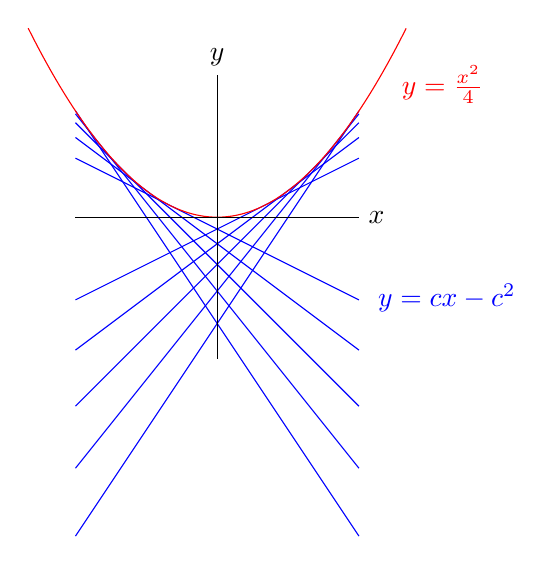
\begin{tikzpicture}[scale=0.6]
  % Curves
  \foreach \c in {-1.5,-1.25,-1,-0.75,-0.5,0.5,0.75,1,1.25,1.5} {
    \draw[blue, domain=-3:3] plot (\x, {\x*\c - \c*\c});
  }
  % Envelope
  \draw[red, domain=-4:4, smooth, samples=100] plot (\x, {\x*\x/4});
  % Axis
  \draw[-] (-3,0) -- (3,0) node[right] {$x$};
  \draw[-] (0,-3) -- (0,3) node[above] {$y$};
  % Labels
  %\foreach \c in {5,10} {
   % \draw (\c/5, -0.1) -- (\c/5, 0.1) node[above] {$\c$};
  %}
   \draw (3.2,-1.7) node[right,blue] {$y=cx-c^2$};
  \draw (3.7,2.8) node[right,red] {$y=\frac{x^2}{4}$};
\end{tikzpicture}$$
\end{sol}
\section{Soluciones singulares}
En las ecuaciones implícitas, pueden existir el siguiente tipo de soluciones.
\begin{defi}
    Una solución de $F(x,y,y')=0$ se llama \textbf{singular} si por cada uno de sus puntos pasa otra solución con la misma pendiente. 
\end{defi}
\begin{eje}
    Considerando la ecuación $y(1+(y')^2)=1$ (la familia de circunferencias que se movían en horizontal $(x-c)^2+y^2=1$) en ningún punto del espacio de soluciones tenemos rectas con misma pendiente, excepto en $y=\pm 1$, que son las soluciones singulares, como vemos a continuación:
$$
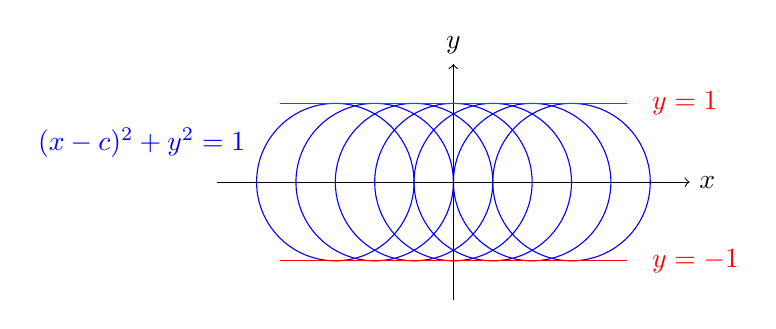
\begin{tikzpicture}[scale=1]
  % Curves
  \foreach \c in {-1.5,-1,...,1.5} {
    \draw[blue] plot[domain=0:2*pi, samples=100] ({\c + cos(\x r)}, {sin(\x r)});
  }
  % Envelope
  \draw[red, domain=-2.2:2.2, smooth, samples=100] plot (\x, 1);
  \draw[red, domain=-2.2:2.2, smooth, samples=100] plot (\x, -1);
  % Labels
  \draw[->] (-3,0) -- (3,0) node[right] {$x$};
  \draw[->] (0,-1.5) -- (0,1.5) node[above] {$y$};
  \draw (-5.4,0.5) node[right,blue] {$(x-c)^2+y^2=1$};
  \draw (2.4,1) node[right,red] {$y=1$};
  \draw (2.4,-1) node[right,red] {$y=-1$};
\end{tikzpicture}$$
\end{eje}
Tengamos la ecuación $F(x,y,p)=0$, veamos cuándo podamos encontrar ecuaciones singulares. Sea $F \in \mc{C}^1$,
\begin{prop}
    Si 
    $$\left\{\begin{array}{l}
         F(x,y,p)=0  \\
         \frac{\partial F}{\partial p}(x,y,p)=0
    \end{array} \right.$$ existen soluciones sigulares. Denominaremos a el sistema anterior curva $p$-discriminante. Las soluciones singulares solo pueden encontrarse entre aquellas curvas $y=\varphi(x)$ que se obtenga eliminando $p$ de la $p$-discriminante. 
\end{prop}
\begin{eje}
    $y(1+p^2)=1$ entonces
    $$p-\text{discriminante } = \left\{ \begin{array}{l}
         y^2(1-p^2)-1=0 \; \Rightarrow \; y^2=1 \; \Rightarrow \; y=\pm 1   \\
         y^2-2p=0 \; \Rightarrow \; p=0
    \end{array}\right.$$
\end{eje}
\begin{ejer}
    Calcular las soluciones singulares de 
    $$y=xy'-(y')^2$$
\end{ejer}
\begin{sol}
    Planteamos la curva $p$-discriminante, es decir, la ecuación
    $$\left\{\begin{array}{lll}
         y=xp-p^2  & & x \dfrac{x}{2}-\left(\dfrac{x}{2}\right)^2=\dfrac{x^2}{4}\\
         0=x-2p \; & \Rightarrow \: p=\dfrac{x}{2} & 
    \end{array} \right.$$
    Luego la única posible solución singular es $y=\dfrac{x^2}{4}$. Comprobemos que 
    \begin{enumerate}
        \item Es solución (Se comprobó anteriormente)
        \item Es singular (si es solución)

        Veamos si por cada uno de sus puntos pasa otra solución con la misma tangente. Sea $(x_o,y_o)=(x_o,\nicefrac{x_o^2}{4})$. Como la otra familia de soluciones es $y=cx-c^2$, ahí buscaremos la que tiene la misma tangente en $(x_o,y_o)$. Esto es, existe $c$ tal que las dos soluciones pasan por el punto y tienen la misma tangente, 
     $$\left\{ \begin{array}{ll}
          \dfrac{x_o^2}{4}=c \cdot x_o-c^2 & = \dfrac{x_o}{2}x_o-\left(\dfrac{x_o}{2}\right)^2=\dfrac{x_o^2}{4} \checkmark \\
          \vspace{-5mm} \\
          \dfrac{x_o}{2}=c
     \end{array}\right.$$
     En consecuencia, $y=\dfrac{x^2}{4}$ es solución singular y no hay otras.
    \end{enumerate}
\end{sol}
\begin{ejer}
    \textbf{26.a)} Resolver con la curva $p$-discriminante $y=2xy'-(y')^2$.
\end{ejer}
\begin{sol}
    $$p-\text{discriminante } = \left\{ \begin{array}{l}
         y=2xp-p^2 \; \Rightarrow \; 2x^2-x^2=x^2   \\
         0=2x-2p \; \Rightarrow \; p=x
    \end{array}\right.$$
    Luego la única posible solución singular es $y=x^2$. En ese caso, la tangentes verificarían $x^2=2x \: 2x-(2x)^2=0$ que no es solución (las hayamos anteriormente), luego no hay soluciones singulares.
\end{sol}
